\documentclass[12pt,letterpaper]{article}
\usepackage{graphicx,textcomp}
\usepackage{natbib}
\usepackage{setspace}
\usepackage{fullpage}
\usepackage{color}
\usepackage[reqno]{amsmath}
\usepackage{amsthm}
\usepackage{fancyvrb}
\usepackage{amssymb,enumerate}
\usepackage[all]{xy}
\usepackage{endnotes}
\usepackage{lscape}
\newtheorem{com}{Comment}
\usepackage{float}
\usepackage{hyperref}
\newtheorem{lem} {Lemma}
\newtheorem{prop}{Proposition}
\newtheorem{thm}{Theorem}
\newtheorem{defn}{Definition}
\newtheorem{cor}{Corollary}
\newtheorem{obs}{Observation}
\usepackage[compact]{titlesec}
\usepackage{dcolumn}
\usepackage{tikz}
\usetikzlibrary{arrows}
\usepackage{multirow}
\usepackage{xcolor}
\newcolumntype{.}{D{.}{.}{-1}}
\newcolumntype{d}[1]{D{.}{.}{#1}}
\definecolor{light-gray}{gray}{0.65}
\usepackage{url}
\usepackage{listings}
\usepackage{color}

\definecolor{codegreen}{rgb}{0,0.6,0}
\definecolor{codegray}{rgb}{0.5,0.5,0.5}
\definecolor{codepurple}{rgb}{0.58,0,0.82}
\definecolor{backcolour}{rgb}{0.95,0.95,0.92}

\lstdefinestyle{mystyle}{
	backgroundcolor=\color{backcolour},   
	commentstyle=\color{codegreen},
	keywordstyle=\color{magenta},
	numberstyle=\tiny\color{codegray},
	stringstyle=\color{codepurple},
	basicstyle=\footnotesize,
	breakatwhitespace=false,         
	breaklines=true,                 
	captionpos=b,                    
	keepspaces=true,                 
	numbers=left,                    
	numbersep=5pt,                  
	showspaces=false,                
	showstringspaces=false,
	showtabs=false,                  
	tabsize=2
}
\lstset{style=mystyle}
\newcommand{\Sref}[1]{Section~\ref{#1}}
\newtheorem{hyp}{Hypothesis}

\title{Problem Set 1}
\date{Due: September 30, 2024}
\author{Applied Stats/Quant Methods 1}

\begin{document}
	\maketitle
	
	
	\vspace{.2cm}
	\section*{Question 1: Education}
	\vspace{.2cm}
A school counselor was curious about the average of IQ of the students in her school and took a random sample of 25 students' IQ scores. The following is the data set:\\


\lstinputlisting[language=R, firstline=15, lastline=16]{PS01.R}  

\vspace{.1cm}

\begin{enumerate}
	\item Find a 90\% confidence interval for the average student IQ in the school.\\
	
	\lstinputlisting[language=R, firstline=18, lastline=28]{PS01.R}  
	
	Results:
	
	\begin{verbatim}
	Mean: 98.44 
	Standard Deviation: 13.09287 
	> class(y)    	 [1] "numeric"
	> length(y) 	[1] 25
	> # 90% confidence interval using t.test
	[1]  93.95993 102.92007
	attr(,"conf.level")
	[1] 0.9
	\end{verbatim}
	
	
	
	
	\vspace{.1cm}
	
	\item Next, the school counselor was curious  whether  the average student IQ in her school is higher than the average IQ score (100) among all the schools in the country.\\ 
	
	\noindent Using the same sample, conduct the appropriate hypothesis test with $\alpha=0.05$.

\vspace{.1cm}

\lstinputlisting[language=R, firstline=39, lastline=41]{PS01.R}  


Results:

\begin{verbatim}
	One Sample t-test
	
	data:  y
	t = -0.59574, df = 24, p-value = 0.7215
	alternative hypothesis: true mean is greater than 100
	5 percent confidence interval:
	102.9201      Inf
	sample estimates:
	mean of x 
	98.44 
\end{verbatim}



	\vspace{.1cm}
Conclusion:
Because the p-value is 0.7215 and it's greater than 0.05, I do not have enough evidence to reject the null hypothesis that average student IQ in the school is equal to the national average of 100 IQ score.


\end{enumerate}

	\vspace{.5cm}


	\section*{Question 2: Political Economy}
	\vspace{.2cm}
\noindent Researchers are curious about what affects the amount of money communities spend on addressing homelessness. The following variables constitute our data set about social welfare expenditures in the USA. \\
\vspace{.5cm}


\begin{tabular}{r|l}
	\texttt{State} &\emph{50 states in US} \\
	\texttt{Y} & \emph{per capita expenditure on shelters/housing assistance in state}\\
	\texttt{X1} &\emph{per capita personal income in state} \\
	\texttt{X2} &  \emph{Number of residents per 100,000 that are "financially insecure" in state}\\
	\texttt{X3} &  \emph{Number of people per thousand residing in urban areas in state} \\
	\texttt{Region} &  \emph{1=Northeast, 2= North Central, 3= South, 4=West} \\
\end{tabular}

\clearpage

\vspace{.7cm}
\noindent Explore the \texttt{expenditure} data set and import data into \texttt{R}.
\vspace{.7cm}

\lstinputlisting[language=R, firstline=54, lastline=70]{PS01.R}  
\vspace{.7cm}

%pritning the table saved using stargazer

% Table created by stargazer v.5.2.3 by Marek Hlavac, Social Policy Institute. E-mail: marek.hlavac at gmail.com
% Date and time: Thu, Sep 26, 2024 - 11:09:05
\begin{table}[!htbp] \centering 
  \caption{} 
  \label{} 
\begin{tabular}{@{\extracolsep{5pt}}lccccc} 
\\[-1.8ex]\hline 
\hline \\[-1.8ex] 
Statistic & \multicolumn{1}{c}{N} & \multicolumn{1}{c}{Mean} & \multicolumn{1}{c}{St. Dev.} & \multicolumn{1}{c}{Min} & \multicolumn{1}{c}{Max} \\ 
\hline \\[-1.8ex] 
Y & 50 & 79.540 & 18.507 & 42 & 129 \\ 
X1 & 50 & 1,911.900 & 400.348 & 1,053 & 2,817 \\ 
X2 & 50 & 281.780 & 118.193 & 111 & 531 \\ 
X3 & 50 & 561.720 & 145.037 & 326 & 899 \\ 
Region & 50 & 2.660 & 1.062 & 1 & 4 \\ 
\hline \\[-1.8ex] 
\end{tabular} 
\end{table} 


\clearpage

\begin{itemize}
\item
Please plot the relationships among \emph{Y}, \emph{X1}, \emph{X2}, and \emph{X3}? What are the correlations among them (you just need to describe the graph and the relationships among them)?
\end{itemize}



	
% Y vs X1
	\begin{figure}[ht]
		\centering
		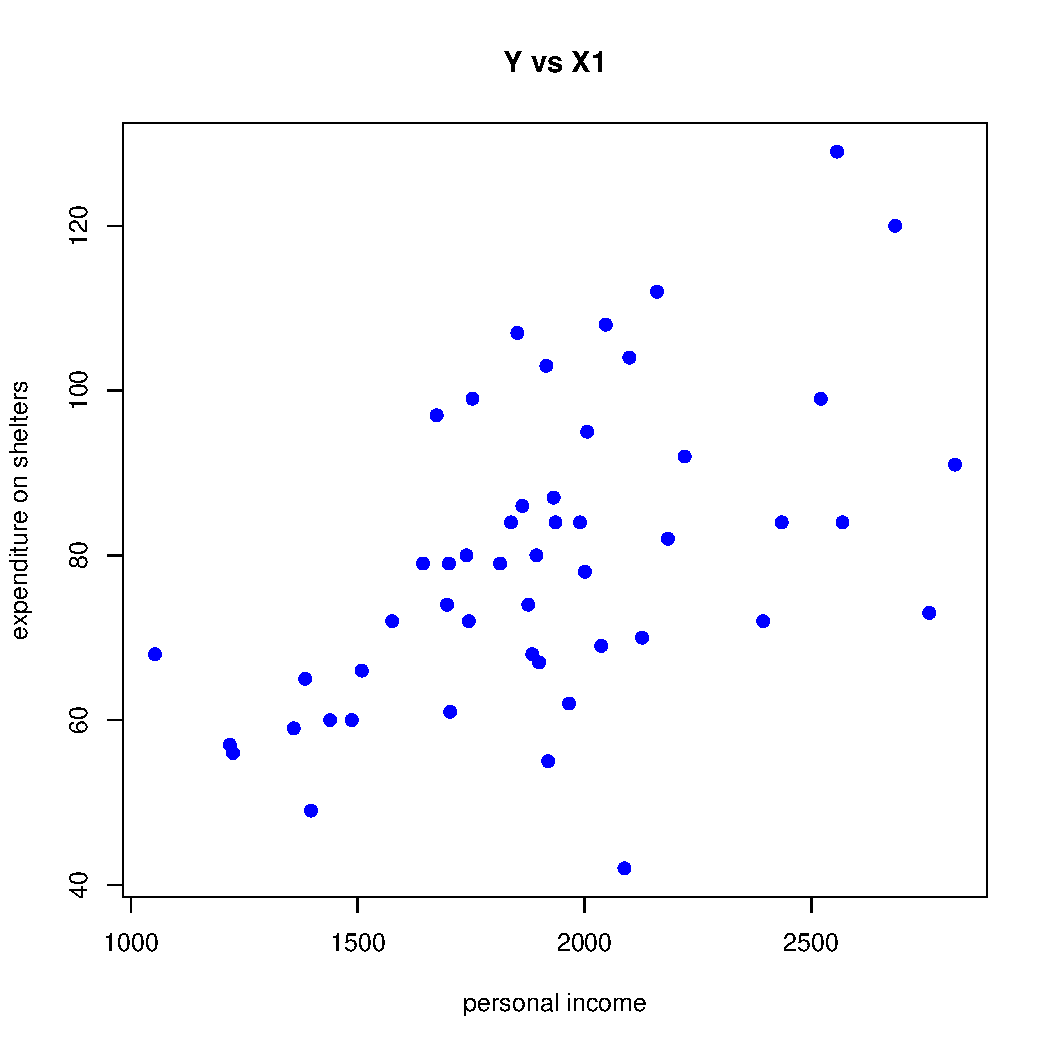
\includegraphics[width=0.40\textwidth]{plot_example1.pdf}
		\center
		There's a correlation between the per capita expenditure in housing assistance regarding the group that has a personal income between 1,600 to 2,100.
	\end{figure}
	
	
	
	
	
% Y vs X2
		\begin{figure}[ht]
		\centering
		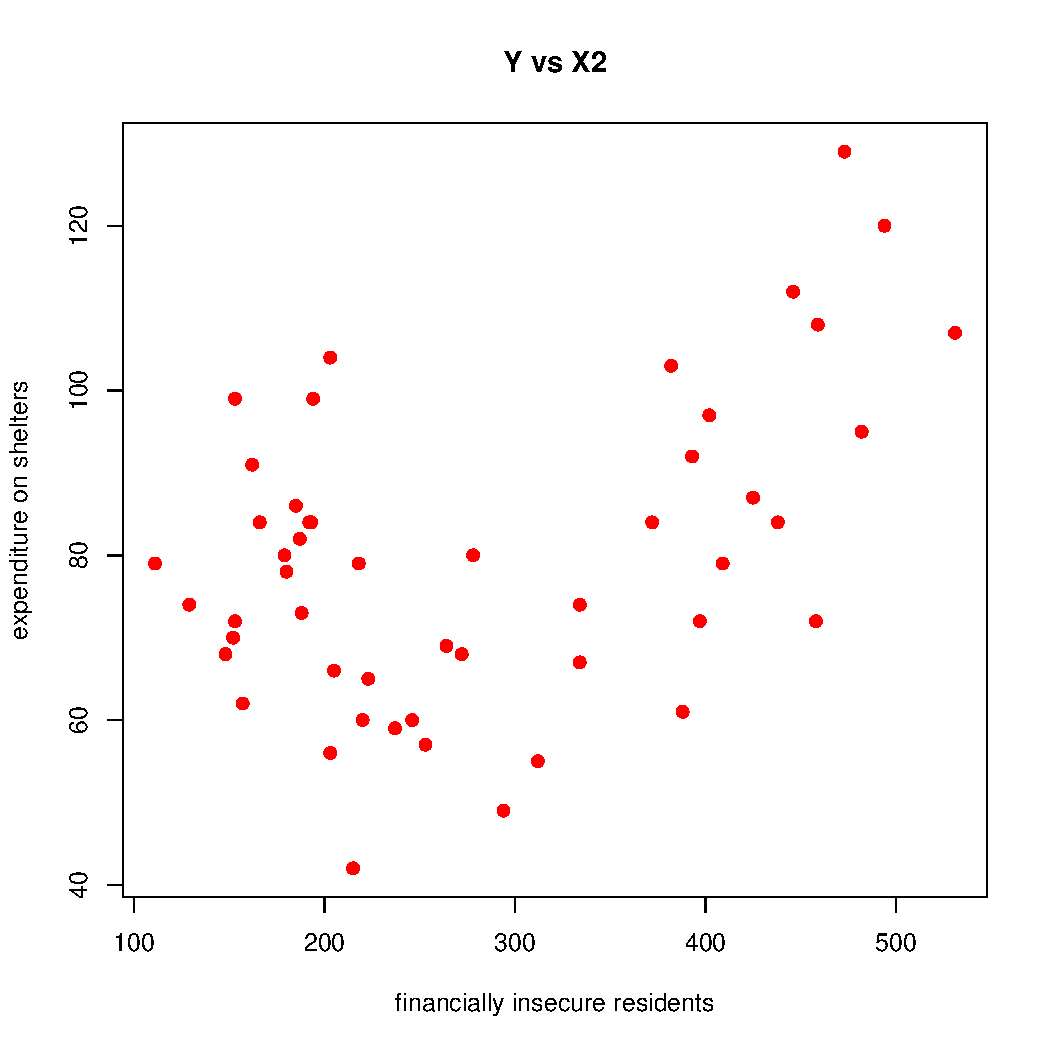
\includegraphics[width=0.39\textwidth]{plot_example2.pdf}
		\center
			The spent per capita for housing assistance is higher where there are more financially insecure residents.
	\end{figure}
	
	
	
	% Y vs X3
	\begin{figure}[ht]
	\centering
	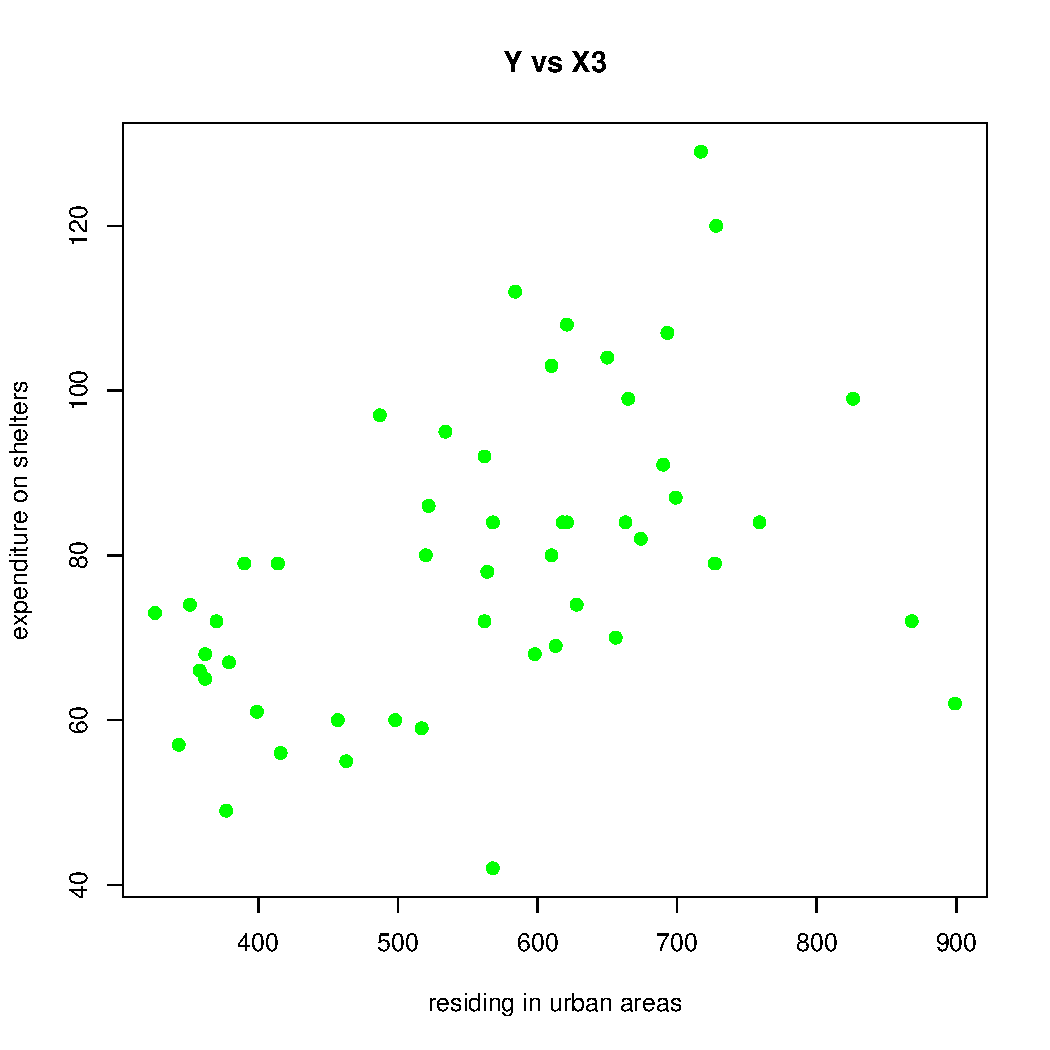
\includegraphics[width=0.45\textwidth]{plot_example3.pdf}
	\center
			The graph shows that spending in housing assistance is lower in rural areas and hight in urban areas.
	\end{figure}
	
	
	
% X1 vs X2
	\begin{figure}[ht]
	\centering
	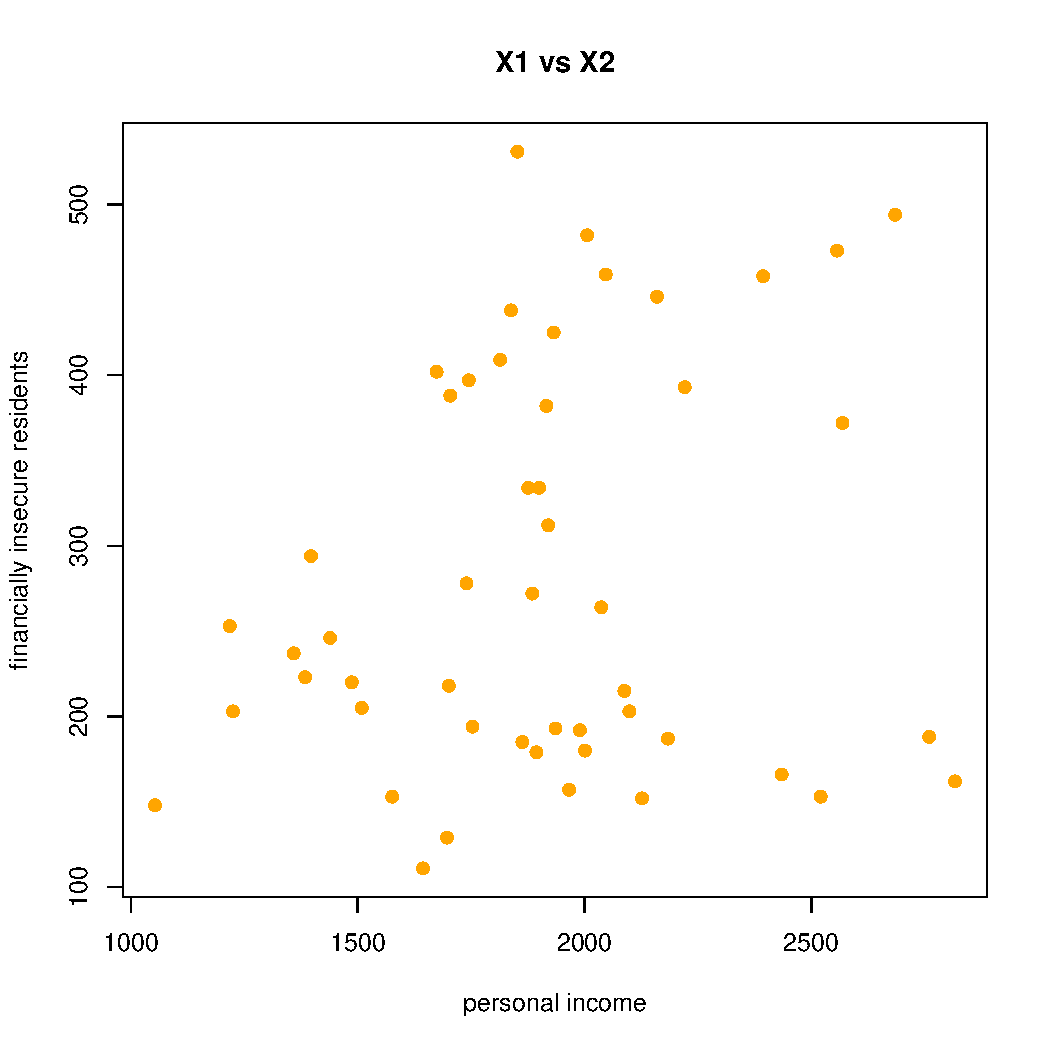
\includegraphics[width=0.45\textwidth]{plot_example4.pdf}
	\center
			The residents with personal income around 1.500 to 2.100 are the ones with a higher financially insecure situation.
	\end{figure}
	

% X1 vs X3
	\begin{figure}[ht]
	\centering
	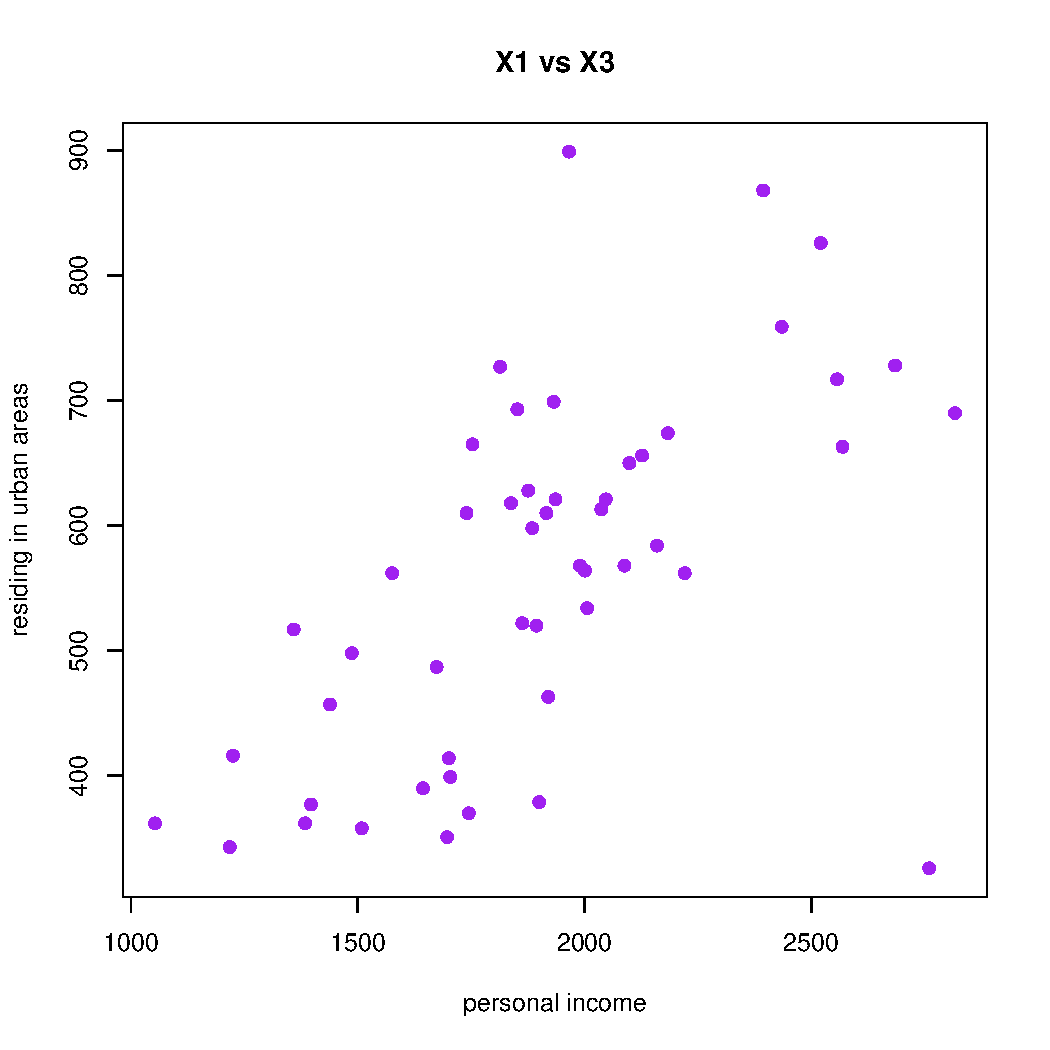
\includegraphics[width=0.45\textwidth]{plot_example5.pdf}
	\center
			People with lower personal income reside un rural areas, and higher incomes in urban areas.
	\end{figure}



% X2 vs X3
	\begin{figure}[ht]
	\centering
	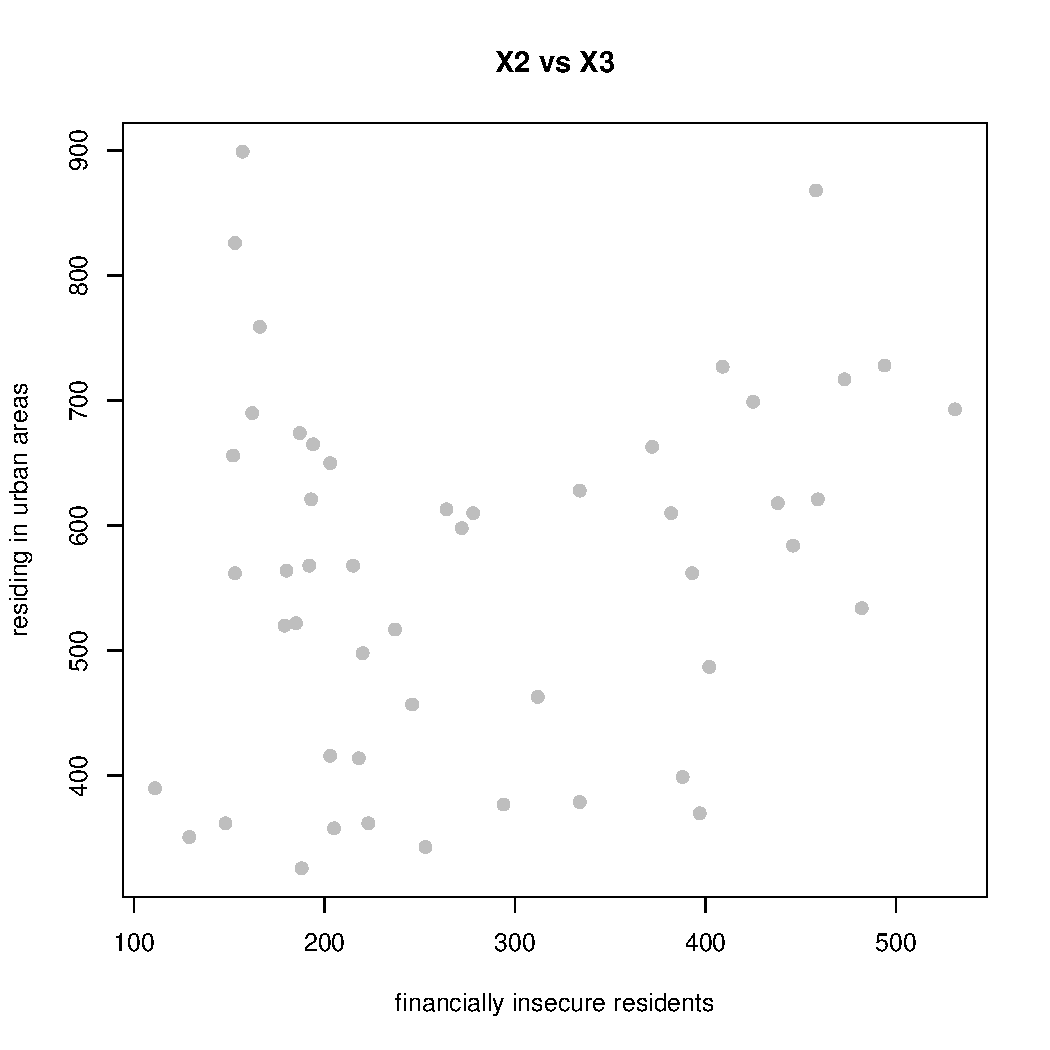
\includegraphics[width=0.45\textwidth]{plot_example6.pdf}
	\center
			Even though people with lower personal incomes live in rural areas, there are less people financially insecure living in rural areas. It may be correct to say that personal income is not related with financial security, and/or the income is lower in rural areas but also the cost of life is cheaper.
	\end{figure}


\clearpage

\begin{itemize}
\item
Please plot the relationship between \emph{Y} and \emph{Region}? On average, which region has the highest per capita expenditure on housing assistance?


% Y vs Region
\begin{figure}[h!]\centering
	\begin{minipage}{0.45\textwidth}  
		\centering
		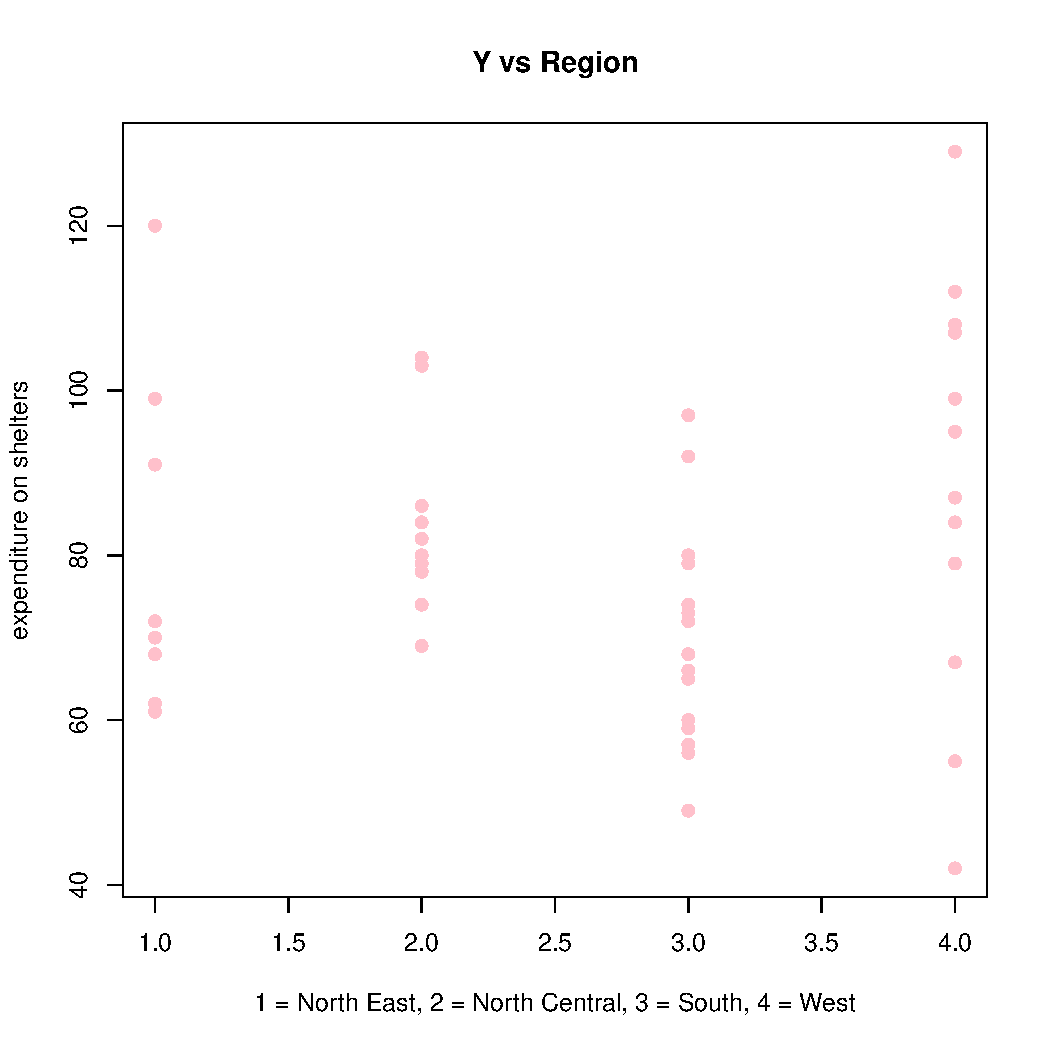
\includegraphics[width=\textwidth]{plot_example7.pdf}
	\end{minipage}\hfill
	\begin{minipage}{0.45\textwidth} 
		\flushleft
		On average, the West region has the highest per capita expenditure on housing assistance.
	\end{minipage}
\end{figure}

\end{itemize}

\vspace{.5cm}

\begin{itemize}
\item
Please plot the relationship between \emph{Y} and \emph{X1}. Reproduce the above graph including one more variable \emph{Region} and display different regions with different types of symbols and colors.


% Y vs X1 vs Region
\begin{figure}[h!]\centering
	\label{fig:plot_1}
	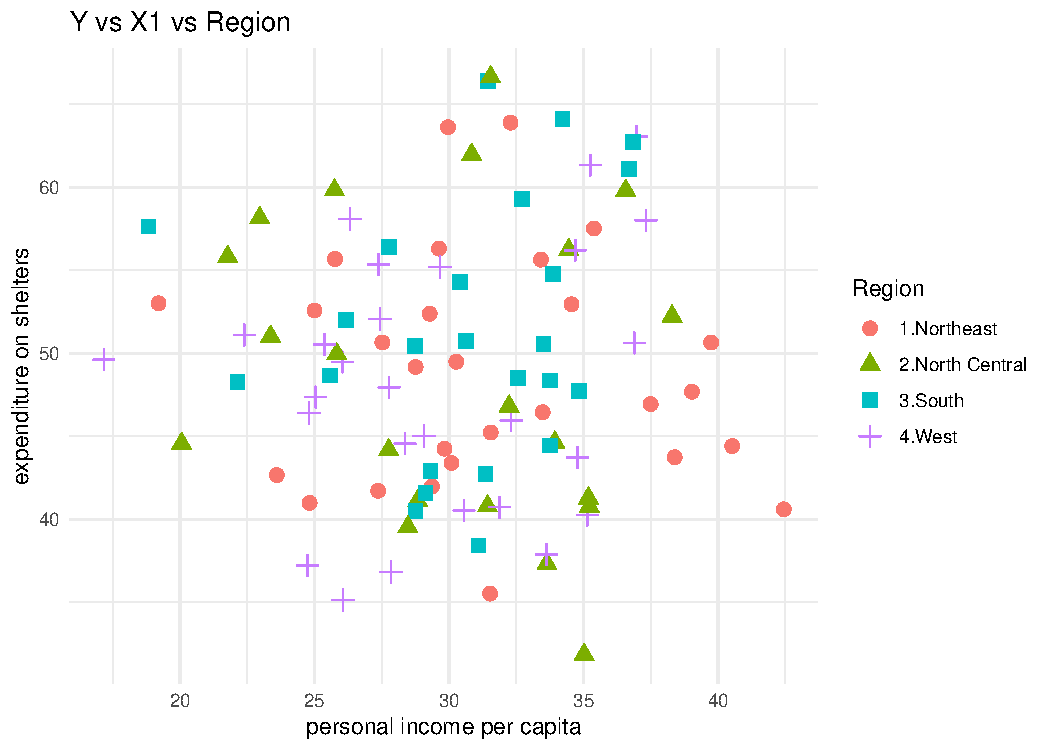
\includegraphics[width=.75\textwidth]{plot_example8.pdf}
\end{figure}

\end{itemize}


\end{document}
